\section{Концепция безопасности БД}
С развитием технологий архитектура программного и аппаратного обеспечения становится только сложнее, что приводит к росту числа их критических уязвимостей. Аналитики компании Embroker прогнозируют, что в период с 2022 по 2025 год бюджеты компаний на информационную безопасность вырастут сразу на 70\%. Это свидетельствует о необходимости усиления мер по защите данных, особенно в контексте увеличивающегося государственного контроля и постоянных новостей о крупных утечках данных \autocite{DataProtectionMaterials}.
Системы управления базами данных (СУБД), в особенности реляционные СУБД и экспертные системы (ЭС), стали доминирующим инструментом в области хранения, обработки и представления данных. Поэтому защита данных от несанкционированного доступа, от несанкционированной модификации или просто от их разрушения является одной из приоритетных задач при проектировании любой информационной системы. Эта проблема (проблема защиты данных) охватывает как физическую защиту данных и системных программ, так и защиту от несанкционированного доступа к данным, передаваемым по линиям связи и находящимся на накопителях, являющегося результатом деятельности как посторонних лиц, так и специальных программ вирусов \autocite[с. 6]{Skakun}.
В этой главе мы рассмотрим основные аспекты безопасности баз данных (БД): какие существуют угрозы для БД, требования по безопасности БД, способы защиты от несанкционированного доступа, защиты от вывода, что означает целостность БД, аудит, многоуровневая защита, какие существуют типы контроля безопасности.

\subsection{Понятие безопасности БД}

\begin{grayquote}
	\textbf{База данных} -- это упорядоченный набор структурированной информации или данных, которые обычно хранятся в электронном виде в компьютерной системе. База данных обычно управляется системой управления базами данных (СУБД). Данные вместе с СУБД, а также приложения, которые с ними связаны, называются системой баз данных, или, для краткости, просто базой данных \autocite{oracleWhatIsDatabase}.
\end{grayquote}


\begin{grayquote}
	Согласно \autocite{CCRFPart4}, базой данных является представленная в объективной форме совокупность самостоятельных материалов (статей, расчетов, нормативных актов, судебных решений и иных подобных материалов), систематизированных таким образом, чтобы эти материалы могли быть найдены и обработаны с помощью электронной вычислительной машины (ЭВМ).
\end{grayquote}

При формулировке основных понятий и определений будем полагать, что защищаемым объектом является не сама БД или экспертная система, а компьютерная система (КС) в целом. Понятие защиты применимо не только к сохраняемым данным. Бреши в системе защиты могут возникать и в других частях системы, например, линии связи, что в свою очередь, подвергает опасности и собственно БД. Следовательно, защита БД должна охватывать используемое оборудование, программное обеспечение, персонал и собственно данные \autocite[сс. 15-18]{Skakun}. 

Информационная безопасность – состояние рассматриваемой КС, при которой она, с одной стороны, способна противостоять дестабилизирующему воздействию внешних и внутренних информационных угроз, а с другой – функционирование системы и сам факт ее наличия не создают угроз для ее пользователей, для внешней среды и для элементов самой КС \autocite[сс. 15-18]{Skakun}.

Защита информации - комплекс мероприятий, направленных на обеспечение информационной безопасности (целостности, доступности, конфиденциальности) \autocite[сс. 15-18]{Skakun}.

Защищаемая информация – информация, являющаяся предметом собственности и подлежащая защите в соответствии с требованиями правовых документов или требованиями, устанавливаемыми собственником информации \autocite[сс. 15-18]{Skakun}. 

Конфиденциальность - это свойство информации быть известной только допущенным и прошедшим проверку субъектам системы \autocite[сс. 15-18]{Skakun}.

Защищаемая информационная система – система, предназначенная для обработки защищаемой информации с требуемым уровнем ее защищенности \autocite[сс. 15-18]{Skakun}.

Система называется безопасной, если она управляет доступом к информации так, что только должным образом авторизованные лица или же действующие от их имени процессы получают право читать, писать, создавать и удалять информацию \autocite[сс. 15-18]{Skakun}. 

Система считается доверенной, если она с использованием достаточных аппаратных и программных средств обеспечивает одновременную обработку информации разной степени секретности группой пользователей без нарушения прав доступа \autocite[сс. 15-18]{Skakun}.

Основными критериями оценки надежности являются политика безопасности и гарантированность \autocite[сс. 15-18]{Skakun}.

Политикой безопасности называют качественное описание комплекса организационно-технологических и программнотехнических мер по обеспечению защиты данных в КС, включает в себя анализ возможных угроз и выбор соответствующих мер противодействия. Выбор конкретных механизмов обеспечения безопасности системы производится в соответствии с политикой безопасности \autocite[сс. 15-18]{Skakun}.

Гарантированность - это пассивный элемент защиты, который отображает меру доверия, которая может быть оказана архитектуре и реализации системы. Гарантированность можно определить тестированием системы в целом и отдельных ее компонентов.

Субъектом доступа называется активный компонент системы, который может стать причиной инициализации потока информации или изменения состояния системы. Субъект представляет собой лицо или процесс, действия которого регламентируются правилами разграничения доступа \autocite[сс. 15-18]{Skakun}. 

Объект доступа - пассивный компонент системы, хранящий, принимающий или передающий информацию, доступ к которой регламентируется правилами разграничения доступа. Объектами доступа в БД является практически все, что содержит конечную информацию: таблицы (базовые или виртуальные), представления, а также более мелкие элементы данных: столбцы и строки таблиц и отдельные поля \autocite[сс. 15-18]{Skakun}. 

Правила разграничения доступа - совокупность правил, регламентирующих права субъектов доступа к объектам доступа. Контроль доступа обязательно включает идентификацию и аутентификацию всех субъектов и их процессов и разграничение полномочий субъектов по отношению к объектам с последующей обязательной проверкой введенных полномочий \autocite[сс. 15-18]{Skakun}.

Идентификация - присвоение объектам и субъектам доступа идентификатора и (или) сравнение предъявляемого идентификатора с перечнем присвоенных идентификаторов \autocite[сс. 15-18]{Skakun}. 

Аутентификация  - проверка принадлежности субъекту доступа предъявленного им идентификатора, подтверждение подлинности \autocite[сс. 15-18]{Skakun}. 

После идентификации и проверки подлинности устанавливается сфера действий субъекта (доступные ему ресурсы КС). Эту процедуру называют авторизацией \autocite[сс. 15-18]{Skakun}.

Авторизация - это предоставление прав (или привилегий), позволяющих их владельцу иметь законный доступ к системе или ее объектам \autocite[сс. 15-18]{Skakun}. 

Привилегия доступа - совокупность прав доступа субъекта доступа \autocite[сс. 15-18]{Skakun}. 

Вышеприведенные понятия в большей степени связаны с организацией защиты конфиденциальных данных. Наряду с защитой конфиденциальных данных в понятие безопасности данных входит также обеспечение целостности и доступности данных \autocite[сс. 15-18]{Skakun}.

Целостность данных - свойство данных сохранять точность и непротиворечивость независимо от внесенных изменений. Зависит от способности информационной системы обеспечить неизменность данных в условиях случайного и (или) преднамеренного искажения (разрушения) \autocite[сс. 15-18]{Skakun}.

Доступность данных - возможность реализации беспрепятственного доступа к информации субъектов, имеющих на это надлежащие полномочия \autocite[сс. 15-18]{Skakun}.

\subsection{Угрозы безопасности БД: общие и специфичные}
Интуитивное понимание угрозы безопасности можно сформулировать как нарушение великолепной тройки: конфиденциальность, целостность, доступность. 
\begin{grayquote}
\textbf{Угроза информационной безопасности} - это осуществляемое или потенциально осуществимое воздействие на компьютерную систему, которое прямо или косвенно может нанести ущерб безопасности информации \autocite[с. 19]{Skakun}.
\end{grayquote}
Уязвимость – свойство информационной системы, обуславливающее возможность возникновения на каком-либо этапе жизненного цикла КС такого ее состояния, при котором создаются условия для реализации угроз безопасности информации. Атакой на КС называют действие, предпринимаемое нарушителем, которое заключается в поиске и использовании той или иной уязвимости \autocite[с. 19]{Skakun}.

По источнику воздействия на КС угрозы разделяются на внутренние и внешние \autocite{Ytebov2008}.

Внешними дестабилизирующими факторами, создающими угрозы безопасности функционированию систем КС, являются:
\begin{itemize}
	\item умышленные, деструктивные действия лиц с целью искажения, уничтожения или хищения программ, данных и документов системы, причиной которых являются нарушения информационной безопасности защищаемого объекта
	\item искажения в каналах передачи информации, поступающей от внешних источников, циркулирующих в системе и передаваемой потребителям, а также недопустимые значения и изменения характеристик потоков информации из внешней среды и внутри системы~\label{pon:pot}
	\item сбои и отказы в аппаратуре вычислительных средств
	\item вирусы и иные деструктивные программные элементы, распространяемые с использованием систем телекоммуникаций, обеспечивающих связь с внешней средой или внутренние коммуникации распределенной системы баз данных
	\item изменения состава и конфигурации комплекса взаимодействующей аппаратуры системы за пределы, проверенные при тестировании или сертификации системы
\end{itemize}

Внутренними источниками угроз безопасности КС являются:
\begin{itemize}
	\item ошибки проектирования КС
	\item ошибки при определении условий и параметров функционирования внешней среды, в которой предстоит использовать информационную систему и, в частности, программно-аппаратные средства защиты данных
	\item ошибки и несанкционированные действия пользователей, административного и обслуживающего персонала в процессе эксплуатации системы
	\item недостаточная эффективность используемых методов и средств обеспечения информационной безопасности в штатных или особых условиях эксплуатации системы
\end{itemize}

Наиболее опасными являются угрозы, вызванные человеческой деятельностью, именно им уделяется особое внимание.

Выше перечислены угрозы на всех уровнях КС~\label{pon:urovs}. Под уровнями будем подразумевать следующее разбиение:
\begin{itemize}
	\item На уровне сети
	\begin{itemize}
		\item Activex-объект
		\item Интерфейсы: OLE DB, ADO, ODBC, JDBC
		\item Протоколы: TCP/IP, IPX/SPX, Named Pipes, Multiprotocol
		\item Рабочие станции
		\item Серверы
		\item Маршрут
		\item URL
	\end{itemize}
	\item На уровне ОС
	\begin{itemize}
		\item Аппаратное обеспечение
		\item Программное обеспечение
		\item Файлы базы данных
		\item Файлы журнала транзакций
		\item Файлы резервного копирования
		\item Transact-SQL, PLSQL
		\item Службы: MSSQLServer, SQLServerАgent, TNSListener и т. д.
	\end{itemize}
	\item На уровне БД
	\begin{itemize}
		\item Пользователи
		\item Роли
		\item Роли приложения
		\item Диаграммы
		\item Представления
		\item Таблицы
		\item Хранимые процедуры
		\item Определения по умолчанию
		\item Правила
		\item Функции
		\item Тип данных
	\end{itemize}
\end{itemize}

Угрозы для КС, делятся на:
\begin{enumerate}
	\item угрозы на уровне ОС
	\item угрозы на уровне сети
	\item угрозы на уровне БД
\end{enumerate}
Атаки на ОС, в которых функционирует СУБД, возникают гораздо чаще, так как защитить ОС гораздо сложнее, чем СУБД. Это обусловлено тем, что число различных типов защищаемых объектов в современных ОС может достигать нескольких десятков, а число различных типов защищаемых информационных потоков -- нескольких сотен. Возможность практической реализации той или иной атаки на ОС в значительной мере определяется архитектурой и конфигурацией ОС. Тем не менее существуют атаки, которые могут быть направлены практически на любые ОС:
\begin{enumerate}
	\item Кража ключевой информации (паролей)
	\item Подбор пароля
	\item Сканирование жестких дисков компьютера
	\item Превышение полномочий
	\item Атаки класса <<Отказ в обслуживании>>
\end{enumerate}
Наиболее опасные атаки на СУБД исходят из сетей. На уровне сетевого
программного обеспечения возможны следующие атаки на СУБД:
\begin{enumerate}
	\item Прослушивание канала
	\item Перехват пакетов на маршрутизаторе
	\item Создание ложного маршрутизатора
	\item Навязывание пакетов
	\item Атаки класса <<Отказ в обслуживании>>
\end{enumerate}

Теперь рассмотрим уровень самой БД. Произведем классификацию по угрозам конфиденциальности, целостности и доступности(согласно \autocite{Ytebov2008}):

Наиболее распространенная угроза для конфиденциальноти - это несанкционированный доступ \autocite[сс. 21]{Skakun}.
Несанкционированный доступ - это  получение пользователем (нарушителем) доступа к объекту в нарушение правил разграничения доступа, установленных в соответствии с принятой в организации политикой безопасности \autocite[сс. 21]{Skakun}.

\begin{itemize}
	\item Несанкционированный доступ к информации можно получить следующими способами~\label{ugr:conf}:
	\begin{enumerate}
		\item Инъекция SQL. Во многих приложениях используется динамический SQL -- формирование SQL-предложений кодом программы путем конкатенации строк и значений параметров. Зная структуру базы данных, злоумышленник может либо выполнить хранимую программу в запросе, либо закомментировать <<легальные>> фрагменты SQL-кода, внедрив, например, конструкцию UNION, запрос которой возвращает конфиденциальные данные. В последнее время злоумышленник может использовать специальные программы, автоматизирующие процесс реализации подобных угроз.

		\item Логический вывод на основе функциональных зависимостей. Пусть дана схема отношения: $R(A_1,\ldots,A_n)$. Пусть $U = \{A_1,\ldots,A_n\}, X ,Y$ -- подмножества из $U$. $X$ функционально определяет $Y$, если в любом отношении $r$ со схемой $R(A_1,\ldots,A_n)$ не могут содержаться два кортежа с одинаковыми значениями атрибутов из $X$ и с различными из $Y$. В этом случае имеет место функциональная зависимость, обозначаемая $X \Rightarrow Y$ . В реальных БД при наличии сведений о функциональных зависимостях злоумышленник может вывести конфиденциальную информацию при наличии доступа только к части отношений, составляющих декомпозированное отношение.

		\item Логический вывод на основе ограничений целостности. Для кортежей отношений в реляционной модели данных можно задать ограничения целостности -- логические условия, которым должны удовлетворять атрибуты кортежей. При этом ограничение целостности может быть задано в виде предиката на всем множестве атрибутов кортежа. В случае попытки изменить данные в таблице, СУБД автоматически вычисляет значение этого предиката, и в зависимости от его истинности операция разрешается или отвергается. Многократно изменяя данные и анализируя реакцию системы, злоумышленник может получить те сведения, к которым	у него нет непосредственного доступа. К этому виду угроз можно отнести также анализ значений первичных/вторичных ключей.

		\item Использование оператора UPDATE для получения конфиденциальной информации. В некоторых стандартах SQL пользователь, не обладая привилегией на выполнение оператора SELECT, мог выполнить оператор UPDATE со сложным логическим условием. Так как после выполнения оператора UPDATE сообщается, сколько строк он обработал, фактически пользователь мог узнать, существуют ли данные, удовлетворяющие этому условию.

		\item Перехват паролей или обход защиты. Перехват паролей обычно осуществляется специально разработанными программами (например, программами-перехватчиками, имитирующими окно ввода пароля и логина).

		\item Маскарад – это выполнение каких-либо действий одним пользователем от имени другого пользователя, обладающего соответствующими полномочиями.

	\end{enumerate}
	\item К угрозам  целостности информации, специфические для СУБД можно отнести следующие~\label{ugr:cel}:
	\begin{enumerate}
		\item С помощью SQL-операторов UPDATE, INSERT и DELETE можно изменить данные в СУБД. Опасность заключается в том, что пользователь, обладающий соответствующими привилегиями, может модифицировать все записи в таблице.
	\end{enumerate}
	\item К угрозам доступности для СУБД можно отнести следующие:
	\begin{enumerate}
		\item Использование свойств первичных и внешних ключей. В первую очередь отнесем сюда свойство уникальности первичных ключей и наличие ссылочной целостности. В том случае, если используются натуральные, а не генерируемые системой значения первичных ключей, может создаться такая ситуация, когда в таблицу невозможно будет вставить новые записи,	так как там уже будут записи с такими же значениями первичных ключей. Если в БД поддерживается ссылочная целостность, можно организовать невозможность удаления родительских записей, умышленно создав подчиненные записи.
		\item Блокировка записей при изменении. Заблокировав записи или всю таблицу, злоумышленник может на значительное время сделать ее недоступной для обновления.
		\item Загрузка системы бессмысленной работой. Злоумышленник может выполнить запрос, содержащий декартовое произведение двух больших отношений. Мощность декартового произведения двух отношений мощности $N_1$ и $N_2$ равна $N_1 \cdot N_2$. Это означает, что при выдаче злоумышленником запроса вида SELECT * FROM Tab1, Tab1 ORDER BY 1, где мощность отношения (количество строк в таблице Tab1) $N_1 = 10000$, мощность результирующего отношения будет $N = N^2_1 = 10000^2$. Вычисление соединения и сортировка результирующего отношения потребуют значительных ресурсов системы и отрицательно скажутся на производительности операций других пользователей.
		\item Использование разрушающих программных средств. Например, атака типа <<троянский конь>> -- запуск пользователями программ, содержащих код, выполняющий определенные действия, внедренный туда злоумышленником.
	\end{enumerate}
\end{itemize}

\subsection{Требования безопасности БД}
Из угроз можно выделить следующий список требований к безопасности БД \autocite{LAPA}:
\begin{itemize}
	\item Функционирование в доверенной среде

	\item Организация физической безопасности файлов данных. Требования к физической безопасности файлов данных СУБД в целом не отличаются от требований, применяемых к любым другим файлам пользователей и приложений

	\item Организация безопасной и актуальной настройки СУБД. Данное требование включает в себя общие задачи обеспечения безопасности, такие как своевременная установка обновлений, отключение неиспользуемых функций или применение эффективной политики паролей

	\item Безопасность пользовательского ПО. Сюда можно отнести задачи построения безопасных интерфейсов и механизмов доступа к данным

	\item Безопасная организация и работа с данными. Вопрос организации данных и управления ими является ключевым в системах хранения информации. В эту область входят задачи организации данных с контролем целостности и другие, специфичные для СУБД проблемы безопасности. Фактически эта задача включает в себя основной объем зависящих от данных уязвимостей и защиты от них
\end{itemize}

Что касается юридических требований, в России пытаются регламентировать эту отрасль, в основном в подобных документах главные мысли про <<безопасную безопасность>>, <<импортозамещение>> и что <<кругом враги>>. Упоминают в них и <<вертикаль власти>> [\autocite{Mysev2019}][\autocite{Elin}].

Для краткого ознакомления можно обратиться к \autocite{CONS149FZ} и в \autocite{CONSUP351}. Более содержательное начинается с \autocite{FSTEKOBKIS}.

Итак, согласно ФСТЭКу автоматизированная система управления, имеет многоуровневую структуру~\label{pon:bez}:
\begin{enumerate}
	\item уровень операторского (диспетчерского) управления (верхний уровень)
	\item уровень автоматического управления (средний уровень)
	\item уровень ввода (вывода) данных исполнительных устройств (нижний (полевой) уровень)
\end{enumerate}

В автоматизированной системе управления объектами защиты являются:
\begin{enumerate}
	\item информация (данные) о параметрах (состоянии) управляемого (контролируемого) объекта или процесса (в том числе входная (выходная) информация, управляющая (командная) информация, контрольно-измерительная информация, иная критически важная (технологическая) информация);
	\item программно-аппаратные средства (в том числе автоматизированные рабочие места, промышленные серверы, телекоммуникационное оборудование, линии связи, программируемые логические контроллеры, производственное, технологическое оборудование (исполнительные устройства));
	\item программные средства (в том числе микропрограммное, общесистемное, прикладное программное обеспечение);
	\item средства защиты информации;
	\item архитектура и конфигурация автоматизированной системы управления.
\end{enumerate}
\begin{grayquote}
	Принимаемые организационные и технические меры защиты информации:
	\begin{itemize}
		\item должны обеспечивать доступность обрабатываемой в автоматизированной системе управления информации (исключение неправомерного блокирования информации), ее целостность (исключение неправомерного уничтожения, модифицирования информации), а также, при необходимости, конфиденциальность (исключение неправомерного доступа, копирования, предоставления или распространения информации)
		\item должны соотноситься с мерами по промышленной, физической, пожарной, экологической, радиационной безопасности, иными мерами по обеспечению безопасности автоматизированной системы управления и управляемого (контролируемого) объекта и (или) процесса
		\item не должны оказывать отрицательного влияния на штатный режим функционирования автоматизированной системы управления.
	\end{itemize}
\end{grayquote}

\begin{grayquote}
	Организационные и технические меры защиты информации, реализуемые в автоматизированной системе управления в рамках ее системы защиты, в зависимости от класса защищенности, угроз безопасности информации, используемых технологий и структурно-функциональных характеристик автоматизированной системы управления и особенностей ее функционирования должны обеспечивать:
	\begin{itemize}
		\item идентификацию и аутентификацию (ИАФ)
		\item управление доступом (УПД)
		\item ограничение программной среды (ОПС)
		\item защиту машинных носителей информации (ЗНИ)
		\item аудит безопасности (АУД)
		\item антивирусную защиту (АВЗ)
		\item предотвращение вторжений (компьютерных атак) (СОВ)
		\item обеспечение целостности (ОЦЛ)
		\item обеспечение доступности (ОДТ)
		\item защиту технических средств и систем (ЗТС)
		\item защиту информационной (автоматизированной) системы и ее компонентов (ЗИС)
		\item реагирование на компьютерные инциденты (ИНЦ)
		\item управление конфигурацией (УКФ)
		\item управление обновлениями программного обеспечения (ОПО)
		\item планирование мероприятий по обеспечению безопасности (ПЛН)
		\item обеспечение действий в нештатных ситуациях (ДНС)
		\item информирование и обучение персонала (ИПО)
	\end{itemize}
\end{grayquote}

Для разнообразия можно ознакомиться с положением дел в Беларуси. Там есть вот такие прикольные законы \autocite{BSEU}:
\begin{itemize}
	\item Об информатизации
	\item О научно-технической информации;
	\item О национальном архивном фонде и архивах в Республике Беларусь
	\item О печати и других средствах массовой информации
	\item О правовой охране программ для ЭВМ и баз данных
	\item О введении в действие Единой системы классификации и кодирования технико-экономической и социальной информации Республики Беларусь
	\item и др.
\end{itemize}

\subsection{Защита от несанкционированного доступа}

В нашем информационном обществе информация является эквивалентом денег. Государства и компании тщательно оберегают ее и охотятся за ней же. Поэтому, говоря о безопасности БД, в первую очередь нужно заботиться о конфиденциальности, а уже потом доступности и целостности. С конфиденциальности и начнем.

Для защиты данных от несанкционированного доступа система должна обеспечивать \autocite[с. 11]{Skakun}:
\begin{itemize}
	\item поддержку определяемых информационной политикой предприятия ограничений прав и полномочий доступа пользователей к данным
	\item защиту от вредоносных действий пользователей, направленных на повреждение данных или получения конфиденциальных данных на основе анализа доступной информации
\end{itemize}

Защита от несанкционированного доступа к данным обеспечивается компьютерными и не компьютерными средствами защиты \autocite[сс. 12-14]{Skakun}.

Компьютерные средства защиты:
\begin{itemize}
	\item идентификация и аутентификации
	\item авторизация пользователей и разграничение доступа
	\item доступ к данным через представления
	\item обновление данных и реализация правил бизнес логики с помощью хранимых процедур, функций и триггеров
	\item резервное копирование и восстановление
	\item обеспечение целостности
	\item управление параллелизмом выполнения транзакций
	\item аудит
	\item шифрование
	\item вспомогательные функции: защита от SQL инъекций, агрегирования и инференции
\end{itemize}

Простейший пример аутентификации это парольная защита. Парольная защита представляет простой и эффективный способ защиты БД от несанкционированного доступа. Пароли устанавлюваются конечным пользователями или администраторами БД и хранятся в определенных системных файлах СУБД в зашифрованном виде. Улучшенным вариантом является использование механизма SSL-аутентификации с использованием сертификатов.

Авторизация пользователей позволяет предоставлять определенные права доступа пользователю, позволяющие их владельцу иметь законный доступ ко всей системе или к ее отдельным объектам.

Представление -- это результат одной или нескольких реляционных операций с базовыми отношениями с целью создания некоторого иного отношения \autocite[с. 12]{Skakun}. Механизм представления является мощным и гибким инструментом организации защиты данных, позволяющим скрыть от определенных пользователей некоторые части БД. В результате пользователи не будут иметь никаких сведений о существовании любых атрибутов или строк данных, которые недоступны через представления, находящиеся в их распоряжении. Представление может быть определено на базе нескольких отношений, после чего пользователю будут предоставлены необходимые привилегии доступа к этому представлению, но не к базовым отношениям. 

К данным, имеющимся в таблице, могут применяться меры защиты по отношению к отдельным полям и отдельным записям. В реляционных СУБД отдельные записи специально не защищаются. Применительно к защите данных в полях таблицы можно выделить такие уровни прав доступа, как полный запрет доступа, только чтение, разрешение всех операций (просмотр, ввод новых значений, удаление, изменение). Более мощным средством защиты данных является их шифрование. Для расшифрования информации пользователи, имеющие санкционированный доступ к зашифрованным данным, имеют ключ и алгоритм расшифрования.

Довольно надежную защиту конфиденциальных данных могут обеспечить методы шифрования. Эти методы включают кодирование информации посредством специального алгоритма, что делает данные непригодными для чтения. Для успешного расшифрования данных требуется знание соответствующего ключа. Уязвимость этого метода состоит в том, что он работает до тех пор, пока злоумышленник не узнает значение ключа.

Для оценки активности использования базы данных производится анализ её журнальных файлов. Эти источники также могут быть задействованы для обнаружения нештатных событий в системе. Периодическое проведение аудиторских проверок, дополненное постоянным мониторингом содержимого журнальных файлов с целью выявления необычной активности в системе, часто способствует своевременному обнаружению и предотвращению попыток нарушения безопасности.

Хранимые процедуры, функции и триггеры представляют собой фрагменты кода на высокоуровневом языке программирования, являющем собой расширение языка SQL, хранящееся и выполняющиеся на сервере. Реализация всех правил бизнес логики с помощью хранимых процедур, функций и триггеров предоставляет значительно более высокий уровень защиты данных, нежели их реализация в клиентских программах.

К не компьютерными средствам защиты относятся:
\begin{itemize}
	\item управление персоналом и общий контроль за физическим доступом
	\item обеспечение защиты помещений и складов с помощью различных охранных систем
	\item заключение гарантийных соглашений и контрактов на обслуживание оборудования и программного обеспечения систем безопасности, поставляемых сторонними поставщиками, что позволяет продлить уверенность в их надежности на определенный период
\end{itemize}

Документы, касающиеся мер безопасности, должны содержать следующее:
\begin{itemize}
	\item область применения данных мер в рамках деловых процессов организации
	\item распределение ответственности и обязанностей между сотрудниками
	\item принятые дисциплинарные меры в случае нарушения установленных ограничений
	\item писок обязательных процедур для выполнения
\end{itemize}

Итак, для минимизации риска несанкционированного доступа необходима реализация комплекса нормативных, организационных и технических защитных мер, в первую очередь: введение ролевого управления доступа, организация доступа пользователей по предъявлению сертификата, выборочное шифрование для сегментов базы данных.

\subsection{Защита от вывода}
Помимо мониторинга, надо внимательно следить за привилегиями (принцип минимальных привилегий) \autocite{Smirnov2007}.
\begin{grayquote}
	Привилегия -- это разрешение на выполнение в системе определенного действия. Не имея соответствующей привилегии, пользователь не может получить доступ к данным или выполнить какое-либо действие.
\end{grayquote}

Все привилегии могут быть разделены на два класса: системные привилегии и привилегии доступа к объектам.

\begin{grayquote}
	Системная привилегия -- это привилегия, которая дает пользователю право на выполнение какой-либо операции в масштабе базы данных. Например, пользователь с системной привилегией ALTER TABLESPACE может изменять любую табличную область (за исключением некоторых ограничений на табличную область SYSTEM).

	Привилегия доступа к объекту -- это разрешение пользователю на выполнение определенной операции над определенным объектом, например выполнение выборки из некоторой таблицы.
	При этом пользователь может формировать любые запросы к данной таблице, но не имеет права модифицировать данные этой таблицы или формировать какой-либо запрос к другой таблице.
\end{grayquote}

\subsection{Целостность БД}
Под понятием целостности данных понимается согласованность информационной модели предметной области с объектами реального мира и их взаимосвязями в каждый момент времени. Любые значительные изменения в предметной области, отраженные в построенной модели, должны также отражаться в базе данных, при этом сохраняя однозначную интерпретацию информационной модели в терминах предметной области. Целостность базы данных не обеспечивает достоверность информации, содержащейся в ней, но гарантирует хотя бы ее правдоподобность, исключая явно невозможные значения. Поэтому важно различать целостность базы данных и достоверность данных. Достоверность (или истинность) данных означает соответствие фактам, хранящимся в базе данных, реальному миру. Контроль целостности данных представляет собой способность системы управления базами данных или самой базы данных в целом обеспечить неизменность данных (т.е. чтобы данные, хранящиеся в системе, соответствовали исходным документам) при случайных или преднамеренных искажениях или разрушениях, иными словами, под целостностью данных подразумевается отсутствие ненадлежащих изменений \autocite[с. 18]{Skakun}.

Мы уже обсуждали основные угрозы целостности в \ref{ugr:cel} на \pageref{ugr:cel}.

Понятие "ненадлежащего изменения" было предложено в работе Д. Кларка и Д. Вильсона. Согласно этому концепту, ни одному пользователю корпоративной системы, включая авторизованных, не следует разрешать изменения данных, которые могут привести к их повреждению или утрате. В их исследованиях определены девять абстрактных теоретических принципов, соблюдение которых способствует обеспечению целостности данных \autocite[сс. 58-59]{Skakun}:

\begin{enumerate}
	\item корректность транзакций
	\item авторизация пользователей
	\item минимизация привилегий
	\item разграничение функциональных обязанностей
	\item аудит произошедших событий
	\item объективный контроль
	\item управление передачей привилегий
	\item эффективное применение механизмов защиты
	\item простота использования защитных механизмов
\end{enumerate}

Средства обеспечения целостности баз данных включают автоматическую поддержку некоторой системы правил, описывающих допустимость и достоверность хранимых и вводимых значений. Реляционная модель включает некоторые характерные правила, вытекающие из существа модели: ограничения домена и ограничения таблицы.
\begin{itemize}
	\item Целостность домена предполагает, что допустимое множество значений каждого атрибута является формально определенным. То есть существуют формальные способы проверки того, что конкретное значение атрибута в базе данных является допустимым. Строка не будет вставлена в таблицу, пока каждое из значений ее столбцов не будет находиться в соответствующем домене (множестве допустимых значений).
	\item Целостность таблицы означает, что каждая строка в таблице	должна быть уникальной. Хотя не все СУБД промышленного уровня требуют выполнения такого ограничения, возможность уникальной идентификации каждой строки представляется необходимой для большинства реальных приложений.
\end{itemize}

Ограничения целостности позволяют гарантировать, что требования к данным будут соблюдаться независимо от способа их загрузки или изменения. В большинстве СУБД предусмотрена поддержка следующих типов статических ограничений целостности\footnote{Немного другая точка зрения: https://studfiles.net/preview/6354061/page:55/}:
\begin{enumerate}
	\item ограничение на определенность значения атрибута (NOT NULL)
	\item ограничение на уникальность значения атрибутов (UNIQUE)
	\item ограничение -- первичный ключ
	\item ограничение -- внешний ключ
	\item ограничение целостности, задаваемое предикатом
\end{enumerate}

На практике наиболее распространены две основные модели обеспечения целостности данных: модель Кларка-Вильсона и модель Биба \autocite[сс. 60-62]{Skakun}.

Модель Кларка-Вильсона была разработана в 1987 году на основе анализа применения бумажного документооборота в коммерческих компаниях. Она представляет собой описательный подход, не включающий строгих математических конструкций. Основные понятия в этой модели - корректность транзакций и разграничение функциональных обязанностей. Модель определяет две категории данных и два класса операций над ними: контролируемые данные (CDI) и неконтролируемые данные (UDI). Правила модели включают обеспечение целостности данных путем применения определенных процедур преобразования и проверки целостности, а также политику разделения обязанностей субъектов. Одним из преимуществ модели является ее простота и легкость интеграции с другими моделями безопасности.

Модель Биба, созданная в 1977 году как модификация модели Белла-ЛаПадулы, также направлена на обеспечение целостности данных. Она использует решетку классов целостности, где базовые правила определяют доступ на чтение и запись в зависимости от уровней целостности субъекта и объекта. Уровни целостности интерпретируются как уровни достоверности, где более высокий уровень безопасности означает более высокую достоверность данных. Модель Биба основана на простых правилах целостности и использовании изученного математического аппарата. Она обладает простотой и хорошо анализируемым математическим описанием, сохраняя при этом некоторые недостатки модели Белла-ЛаПадулы.

\subsection{Аудит безопасности}

Данный подразрадел является переводом и резюме 9 главы книги Database Security \autocite{DatabaseSecurity}.

\subsubsection{Определение}

Аудит информационной безопасности информационных систем — это процесс оценки системы защиты информации на предмет соответствия стандартам и требованиям безопасности, а также выявления уязвимостей и возможных угроз безопасности.

\subsubsection{Цели проведения аудита}

Основной целью проведения аудита информационной безопасности является выявление уязвимостей в системе защиты информации и предотвращение возможных угроз безопасности. Кроме того, аудит также позволяет определить эффективность системы защиты, а также проверить соответствие информационных систем законодательству и стандартам безопасности.

\subsubsection{Процесс проведения аудита}

Процесс проведения аудита обычно включает 3 этапа:
\begin{enumerate}
	\item Подготовка и планирование
	\item Аудит
	\item Отчет
\end{enumerate}

\paragraph{1. Подготовка и планирование.}

На этом этапе формируется команда, которая будет проводить аудит, определяется область аудита, составляется план и график проведения аудита.

Область аудита — это система, на которой будет сосредоточен аудит. Определяются приоритетные активы и периметр аудита. Связанные активы изучаются и классифицируются как находящиеся в периметре аудита или за его пределами. Определение области аудита требует от аудитора четкого понимания устройста инфраструктуры и организационной структуры. Список активов должен быть составлен путем анализа документации, архитектуры системы и организационных иерархий. Должны быть включены как материальные (например, компьютеры, серверы, принтеры, отдельные лица), так и нематериальные (например, данные, электронная почта, веб-приложения, пароли) элементы. Угрозы этим активам должны быть идентифицированы, а приоритизация осуществляется с использованием результатов анализа рисков. Хорошей практикой является проверка результатов предыдущего аудита безопасности, чтобы понять, какие приоритеты были расставлены в прошлом.

После определения области аудита можно четко определить цели аудита и составить план. План составляется с учетом уже собранной информации, а также с учетом даты и времени проведения аудита, стратегии резервного копирования и влияния процесса на ежедневные операции.

Из-за множества компонентов системы (например, файлов, серверов, приложений, данных) и методов (например, политик, межсетевых экранов, биометрии, шифрования), задействованных в обеспечении безопасности, практически невозможно провести аудит всей системы одновременно. Поэтому в разное время года для организации планируются несколько небольших аудитов безопасности, каждый из которых фокусируется только на определенной области. Обычная разбивка областей аудита безопасности включает в себя физическую безопасность, безопасность ОС, веб-приложений, веб-серверов, серверов БД, сетевого оборудования, политик и процедур.

График проведения аудита может сильно измениться, если резко меняются приоритеты. Например, в таблице на Рис. 1 представлен возможный график аудита безопасности для организации. В первом столбце таблицы отображается исходный график аудита, а во втором столбце отображается тот же график после внесения корректировок из-за обнаружения уязвимости (возможной SQL-инъекции).

\begin{figure}[h!]
    \centering
    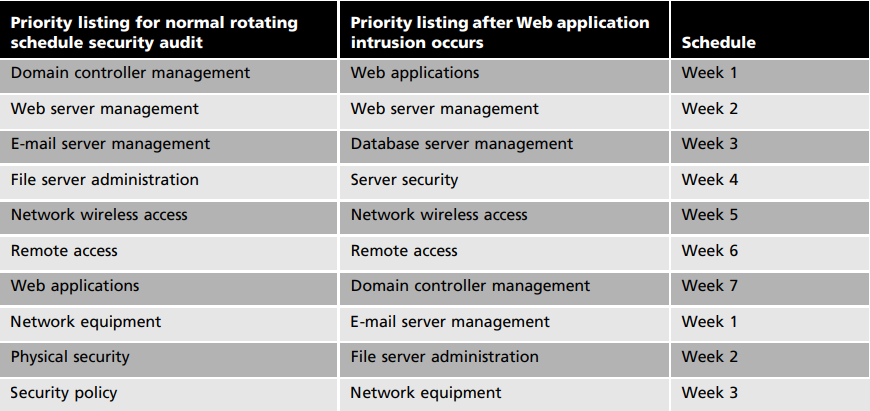
\includegraphics[width=0.8\textwidth]{assets/Schedule_audit}
    \caption{Пример графика проведения аудита}
\end{figure}

\paragraph{2. Аудит.}

На этом этапе подробный план аудита безопасности, составленный на предыдущем этапе, приводится в действие. Конкретные действия во время проведения аудита зависят от множества факторов, включая тип аудита, область аудита и организацию. Очевидно, что аудит, предназначенный для проверки физической безопасности, будет включать в себя совершенно иные действия, чем аудит, предназначенный для проверки администрирования СУБД. На Рис.2 в таблице показан список действий, которые обычно выполняются в процессе аудита для разных типов систем.

\begin{figure}[h!]
    \centering
    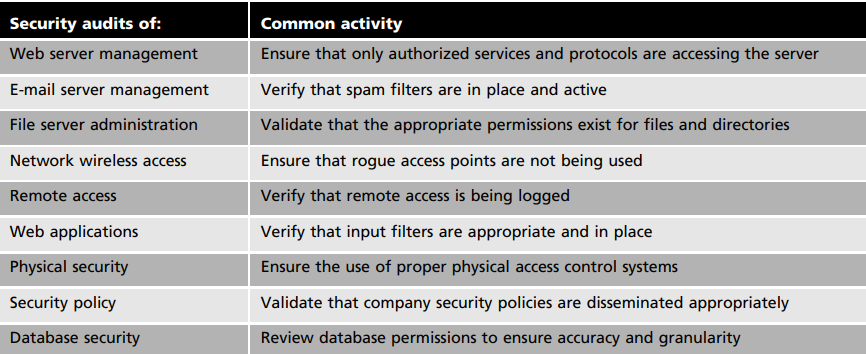
\includegraphics[width=0.8\textwidth]{assets/Common_actions_audit}
    \caption{Пример обычных действий при проведении аудита}
\end{figure}

\paragraph{3. Отчет.}

Заключительным этапом процесса аудита безопасности является подведение итогов, на котором аудитор или комитет аудиторов устно и письменно сообщает о результатах аудита.

Во всех аудиторских отчетах можно обнаружить некоторые важные общие черты, включающие исходную информацию, определенную область аудита, план и цель аудита, ключевые выводы, используемую для риск-аналитики методологию, рекомендации по устранению найденных уязвимостей.

\subsubsection{Процесс проведения аудита БД}

\paragraph{Подготовка и планирование аудита БД.}

Подготовка к аудиту безопасности БД требует, чтобы аудитор собрал как можно больше информации об инфраструктуре БД для четкого определения периметра аудита. Периметр должен включать подробную информацию о людях, данных, технологиях и документах, которые будут играть роль в рамках конкретного аудита. На Рис. 3 представлен пример периметра аудита БД.

Сбор информации включает в себя консультацию с администраторами БД, изучение схем баз данных, архитектуру сети, политик и процедур, связанных с БД. Часто организации имеют несколько СУБД, поэтому необходимо принять решение, сколько систем будет проверяться.

\begin{figure}[h!]
    \centering
    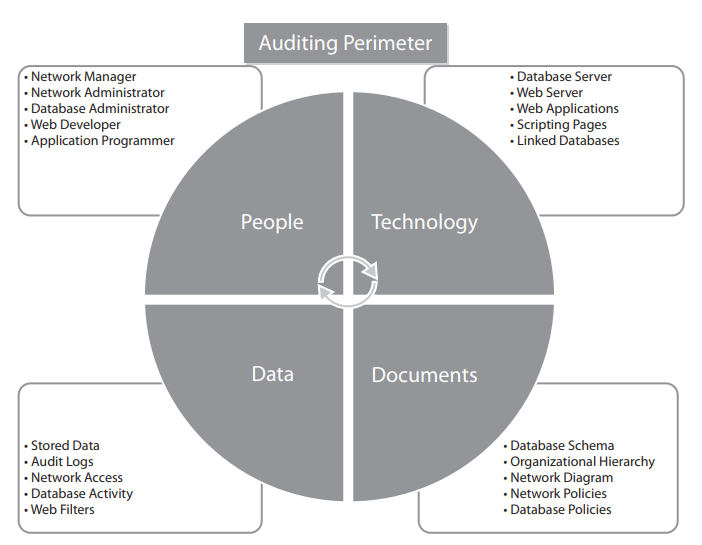
\includegraphics[width=0.8\textwidth]{assets/DB_audit_perimeter}
    \caption{Пример периметра аудита БД}
\end{figure}

На этом этапе также необходимо получить понимание функциональности, назначения и структуры всех используемых СУБД. Важна такая информация, как вендор СУБД, ОС функционирования СУБД, стратегия резервного копирования. Необходимо провести анализ данных на предмет связи с организационной иерархией, чтобы понять потребности сотрудников в хранении данных и манипулировании ими.

Анализ рисков и угроз является еще одним важным этапом планирования аудита БД, поскольку он помогает определить приоритетный список действий, который можно использовать в качестве отправной точки для аудита. Чтобы гарантировать, что были приняты все меры для защиты БД и учтены все риски, необходимо рассматривать всю инфраструктуру БД, в том числе сетевую.

Аудит БД может выполняться одним из двух способов. Аудитор может сначала сосредоточиться на компонентах, связанных с БД (например, веб-приложениях, веб-серверах, middleware, скриптах), прежде чем переходить к БД, или аудит может начаться с БД, и впоследствии проводится проверка связанных компонентов.

\paragraph{Аудит БД.}

Из-за большого количества ресурсов, необходимых для проверки всей инфрастуктуры БД, аудит обычно проводится частями, фокусируясь на конкретных функциях или компонентах. Эти части могут включать обслуживание серверов, администрирование учетных записей, контроль доступа, привилегии доступа к данным, пароли, шифрование, активность пользователей.

\paragraph{Обслуживание серверов.}

Аудит обслуживания сервера включает проверку стратегий резервного копирования, контроля обновлений и версий ПО, управления ресурсами и обновлениями оборудования. Ниже приведен список примеров аудиторских проверок:

\begin{enumerate}
	\item Установлены последние патчи безопасности СУБД
	\item Установлены последние критические обновления СУБД
	\item Используемая версия СУБД поддерживается
	\item Существует и используется процедура обновления СУБД
	\item Существует и применяется политика резервного копирования, включающая аварийное восстановление
	\item Существует и используется процедура проверки резервных копий
\end{enumerate}

\paragraph{Администрирование учетных записей.}

Аудит администрирования учетных записей включает проверку того, как администратор управляет учетными записями пользователей, а именно: создание, удаление учетных записей пользователей; применение политик безопасности; назначение групп, ролей и привилегий. Примеры аудиторских проверок:

\begin{enumerate}
	\item Различные роли администраторов четко определены
	\item Учетные записи администраторов распределяются согласно политике
	\item Неактивные или ненужные учетные записи пользователей удаляются
	\item Общие учетные записи не используются
	\item Учетные записи по умолчанию отключены или удалены
\end{enumerate}

\paragraph{Контроль доступа.}

Контроль доступа включает отслеживание доступа пользователей к БД. Контроль доступа необходим для обеспечения конфиденциальности, целостности и доступности СУБД. Примеры аудиторских проверок:

\begin{enumerate}
	\item Только доверенные IP-адреса могут получить доступ к базе данных
	\item Доступ к конфиденциальным данным имеют только те, кому они необходимы
	\item Администраторы не имеют возможности удаленно вносить изменения в БД без дополнительной аутентификации
	\item Доступ к резервным копиям и аварийному восстановлению разрешен только администраторам
\end{enumerate}

\paragraph{Привилегии доступа к данным.}

Обеспечение соответствия привилегий доступа во время аудита — трудоемкая задача, которая требует сотрудничества с сетевым администратором. Примеры аудиторских проверок:

\begin{enumerate}
	\item PUBLIC удален из системы
	\item Неявное предоставление привилегий тщательно рассматривается
	\item Используется принцип наименьших привилегий
	\item Привилегии учетной записи в операционной системе ограничены
\end{enumerate}

\paragraph{Пароли.}

Надежные пароли имеют решающее значение в доверенной среде, поскольку они представляют собой первую линию защиты, с которой столкнутся злоумышленники. Большинство СУБД можно настроить так, чтобы пароли автоматически соответствовали определенной политике. Аудит управления паролями включает проверку написанной политики, конфигурации сервера и учетных записей пользователей по умолчанию. Примеры аудиторских проверок:

\begin{enumerate}
	\item Опции управления паролями включены в СУБД
	\item Парольная политика включает спецификации для неудачных входов в систему, устаревания, сложности, истории, срока действия и содержимого
	\item Пароли по умолчанию должны быть изменены
	\item По возможности пароли не хранятся в БД
	\item Пароли шифруются с использованием стойкого шифрования, если они хранятся в БД
\end{enumerate}

\paragraph{Шифрование.}

Шифрование должно быть проверено как для хранящихся, так и для перемещаемых данных по БД. Примеры аудиторских проверок:

\begin{enumerate}
	\item Перемещаемые данные шифруются с использованием надежных методов шифрования
	\item Для шифрования данных используются симметричные ключи
	\item Шифрование настроено точно согласно политике
\end{enumerate}

\paragraph{Активность пользователей.}

Должен быть настроен мониторинг действий пользователей, работающих с СУБД. Примеры аудиторских проверок:

\begin{enumerate}
	\item Неудачные входы отслеживаются
	\item Неудачные запросы отслеживаются
	\item Изменения метаданных отслеживаются
\end{enumerate}

\paragraph{Отчет об аудите БД.}

Подготовка и презентация отчета об аудите БД совпадает с описанным ранее общим этапом аудита безопасности.

\clearpage

\subsection{Многоуровневая защита}
Уже было сказано про уровни в связке сеть-ОС-БД [\ref{pon:urovs}] и уровни ФСТЭК-а [\ref{pon:bez}].

Анализ наиболее успешных решений в области обеспе­чения информационной безопасности баз данных позволил сформулировать несколько полезных принципов, которыми можно руководствоваться при проектировании систем защиты \autocite{Smirnov2007}:
\begin{itemize}
	\item экономическая оправданность механизмов защиты
	\item открытое проектирование
	\item распределение полномочий между различными субъектами в соответствии с правилами организации
	\item минимально возможные привилегии для пользователей и администраторов
	\item управляемость системы при возникновении отказов и сбоев
	\item психологическая приемлемость работы средств защиты данных
\end{itemize}

Многоуровневую модель защиты данных может реализовать мандатный (заметим, что есть также дискреционная и ролевая модель безопасности) принцип построения системы разграничения доступа в СУБД.

Ключевые аспекты мандатного подхода к разграничению доступа, включая следующие принципы:
\begin{itemize}
	\item каждый субъект и объект должны быть четко идентифицированы
	\item существует упорядоченный набор меток конфиденциальности и соответствующих им уровней доступа, начиная от общедоступных объектов до наиболее конфиденциальных
	\item каждому объекту присваивается метка конфиденциальности, а каждому субъекту – степень доступа
	\item доступ к чтению информации из объекта разрешается только субъекту, чья степень доступа не ниже метки конфиденциальности объекта
	\item доступ к записи информации в объект разрешается только субъекту, чья метка конфиденциальности не выше метки объекта. Это также означает, что информация, записанная субъектом, автоматически получает уровень классификации субъекта
	\item в течение своего существования каждый субъект имеет уровень конфиденциальности, равный максимальной метке конфиденциальности объектов, к которым он имеет доступ
\end{itemize}

К преимуществам мандатного разграничения доступа включают более высокую надежность работы системы и большую простоту определения правил доступа по сравнению с дискреционным разграничением.

\subsection{Типы контроля безопасности: потоковый, контроль вывода, контроль доступа}
Про все три типа мы уже поговорили. В частности \ref{pon:pot} и \ref{pon:bez}. Единственное, что осталось уточнить -- это контроль доступа. 

Управление доступом представляет собой стратегию обеспечения безопасности информации, осуществляемую через контроль и регулирование использования ресурсов системы, таких как элементы базы данных, программное обеспечение и технические средства. Эта стратегия включает следующие ключевые функции защиты \autocite[с. 36]{Skakun}:
\begin{enumerate}
	\item идентификация пользователей и ресурсов системы
	\item проверка подлинности объекта или субъекта на основе предъявленного идентификатора (аутентификация)
	\item ограничение доступа и проверка полномочий (авторизация), обеспечивающие соблюдение установленных регламентов
	\item фиксация обращений к защищаемым ресурсам (протоколирование и аудит)
	\item реакция на попытки несанкционированного доступа
\end{enumerate}
То есть, идейно он этот вопрос распадается на два: \textit{кому} и \textbf{что} мы будем разрешать?

\paragraph{Кому?}

Получение доступа к ресурсам информационной системы предусматривает выполнение трех процедур: идентификации, аутентификации и авторизации.

Общепринято, что технологии идентификации и аутентификации являются обязательным элементом защищенных систем, так как обеспечивают аксиоматический принцип персонализации субъектов и, тем самым, реализуют первый (исходный) программ­но-технический рубеж защиты информации в компьютерных системах.

\begin{enumerate}
	\item Сущность процедуры идентификации состоит в назначении пользователю, т. е. объекту -- потребителю ресурсов сервера баз данных -- имени. Имя пользователя -- это некоторая уникальная метка, соответствующая принятым соглашениям именования и обеспечивающая однозначную идентификацию объекта реального мира в пространстве отображаемых объектов. С позиций ИС источники, предъявившие идентификатор, неразличимы.
	\item Сущность процедуры аутентификации состоит в подтверждении подлинности пользователя, представившего идентификатор.
	\item Сущность процедуры авторизации состоит в определении перечня конкретных информационных ресурсов, с которыми аутентифицированному пользователю разрешена работа.

\end{enumerate}
Процедуры идентификации, аутентификации и авторизации являются обязательными для любой защищенной ИС.

\paragraph{Что?}
Обычно используют одну из трех моделей безопасности: дискреционная, мандатная и ролевая.
\begin{enumerate}
	\item Простейшая (одноуровневая) модель безопасности данных строится на основе дискреционного (избирательного) принципа разграничения доступа, при котором доступ к объектам осуществляется на основе множества разрешенных отношений доступа в виде троек -- <<субъект доступа -- тип доступа -- объект доступа>>.

	Наглядным и распространенным способом формализованного представления дискреционного доступа является матрица доступа, устанавливающая перечень пользователей (субъектов) и перечень разрешенных операций (процессов) по отношению к каждому объекту базы данных (таблицы, запросы, формы, отчеты).

	\item Мандатная модель доступа характерна для случая, когда возможность конкретных действий с данными или документами определяется внешним, обычно глобальным собственником информации. Исторически в роли такого глобального собственника чаще всего выступало государство. Основная идея мандатной модели доступа состоит в приписывании объектам и субъектам доступа меток. Если метки объекта и субъекта соответствуют (в некотором смысле), то субъект получает право на выполнение определенных действий с объектом. В роли метки, приписываемой субъектам в государственных структурах, выступает, например, форма допуска. В реляционной модели в качестве структуры, обладающей меткой, естественно выбрать кортеж.

	\item В основу ролевой модели положена идея принадлежности всех данных системы некоторой организации, а не пользователю, как в случае моделей дискреционного и мандатного доступа. В целом модель ориентирована на упрощение и обеспечение формальной ясности в технологии обеспечения политики безопасности системы. Управление доступом в ролевой модели осуществляется как на основе матрицы прав доступа для ролей, так и с помощью правил, регламентирующих назначение ролей пользователям и их
	активацию во время сеансов.

	В ролевой модели классическое понятие субъект разделяется на две части: пользователь и роль. Пользователь — это человек, работающий с системой и выполняющий определенные служебные обязанности. Роль -- это активно действующая в системе абстрактная сущность, с которой связан ограниченный, логически связанный набор привилегий, необходимых для осуществления определенной деятельности. (Самым распространенным примером роли явля­ется присутствующая почти в каждой системе учетная запись администратора (например, root для UNIX и Administrator для Windows), который обладает специальными полномочиями и может использоваться несколькими пользователями.

	Ролевая модель включает три компонента: модель отображения пользователь -- роль, модель отображения привилегия -- роль и модель отображения роль -- роль. Для упрощения логической структуры объектов управления вводится понятие иерархии ролей. Роль, входящая в иерархию, может включать другие роли, наследуя все привилегии включаемых
	ролей.
\end{enumerate}
\clearpage
